% BrailleLens --- CS3501 Group 15 research paper
% Overleaf: Menu → Compiler → pdfLaTeX  |  Main document → main.tex
% Upload this folder (or this file alone) as a new Overleaf project.
\documentclass[conference]{IEEEtran}

\IEEEoverridecommandlockouts
\usepackage{cite}
\usepackage{amsmath,amssymb,amsfonts}
\usepackage{algorithm}
\usepackage{algpseudocode}
\usepackage{graphicx}
\usepackage{textcomp}
\usepackage{xcolor}
\usepackage{booktabs}
\usepackage{multirow}
\usepackage{tabularx}
\usepackage{array}
\usepackage{tikz}
\usetikzlibrary{arrows.meta,positioning,fit,calc,shapes.geometric,decorations.pathreplacing}
\usepackage{hyperref}
\usepackage{url}
\usepackage{balance}
\usepackage{microtype}

\hypersetup{
  colorlinks=true,
  linkcolor=black,
  citecolor=black,
  urlcolor=blue
}

\def\BibTeX{{\rm B\kern-.05em{\sc i\kern-.025em b}\kern-.08em
    T\kern-.1667em\lower.7ex\hbox{E}\kern-.125emX}}

\title{BrailleLens: Real-Time Optical Braille Recognition
with YOLO26 Fingertip Tracking for Interactive Sinhala Literacy}

\author{
\IEEEauthorblockN{Group 15}
\IEEEauthorblockA{\textit{CS3501 Data Science and Engineering Project}\\
\textit{BrailleLens}\\
% Fill in names and affiliation before submission.
}
}

\begin{document}

\maketitle

\begin{abstract}
Optical Braille recognition (OBR) is typically evaluated on flatbed scans of
English or Chinese pages, yet literacy support for Sinhala Braille readers
requires a system that works from a handheld camera, survives lighting and
perspective shift, and can name the cell under a moving fingertip. We present
\textbf{BrailleLens}, a two-stage OBR pipeline coupled to an interactive
fingertip reader. A single-class YOLO26 detector localises Braille
\textit{cells} (not individual dots); a compact 64-class convolutional network
classifies each $64\times 64$ crop into a language-agnostic 6-dot code; a
deterministic two-pass decoder then maps codes to Sinhala (or English).
Fingertip contact is tracked by a Braille-domain YOLO26n detector as the
default, with a classical YCrCb skin-contour estimator as a per-frame
fallback when the network returns no box. A still, hand-free frame is
auto-captured into a CellMap; subsequent frames are aligned by ORB+RANSAC
homography so a dwell on a cell can announce its character. On public
scanner data the classifier reaches 99.24\% cell accuracy after
normalisation and fine-tuning. On a held-out Sinhala Gold set, gold-domain
fine-tuning lifts classifier accuracy from 67.7\% to 95.9\% and cell-detector
mAP$_{50}$ from 0.41 to 0.80; end-to-end letters-only page accuracy is
79.3\%. The domain-adapted fingertip model reports mAP$_{50}=0.995$ on a
small Braille-fingertip test split. We analyse failure modes unique to
open-book photography (spine foreshortening, decorative ruler rows, crop-box
geometry) and release the full data-to-live-app stack as a course-scale
research system.
\end{abstract}

\begin{IEEEkeywords}
Optical Braille recognition, YOLO26, fingertip tracking, Sinhala Braille,
domain adaptation, assistive reading, convolutional neural networks
\end{IEEEkeywords}

\section{Introduction}
\label{sec:intro}

Grade-1 Braille encodes each character as a $2\times 3$ matrix of raised
dots. For a sighted teacher, a parent, or a late learner, those dots are
hard to read at a glance; for a Sinhala learner they are harder still,
because Sinhala Braille uses a two-cell indicator system for combining
vowel signs that has no one-to-one Latin analogue~\cite{unicode-sinhala}.
Existing OBR systems~\cite{li2018dsbi,ovodov2021obr} largely assume a
flatbed scan, a known page language, and a full-page transcription
objective. They do not answer the question a learner actually asks while
touching a page: \emph{what is the character under my finger, right now?}

BrailleLens is built around that question. A phone or webcam looks down onto
an open book. When the camera is still and the hand is off the page, the
system freezes a frame, detects every Braille cell, classifies it, and
builds a geometric CellMap. When the finger returns, a domain-tuned YOLO26
fingertip detector (with a skin-contour fallback) reports a contact point;
an exponential moving average rejects teleports; an ORB homography maps the
live tip back into the scan's coordinate frame; a dwell filter fires only
after the same cell is held for a few seconds. Learning mode announces the
character; testing mode quizzes it.

This design is forced by the data, not by taste. A 64-class CNN trained only
on synthetic cells scores 100\% on synthetic test images and 51.2\%
zero-shot on the DSBI scanner test set~\cite{li2018dsbi}---a classic domain
gap. Fine-tuning on 26 DSBI train pages closes it to 98.4\% (99.2\% with
per-crop normalisation). The same CNN, given ground-truth boxes on the
handheld Angelina photographs~\cite{ovodov2021obr}, exceeds 99\%, but
end-to-end transcription through classical dot clustering collapses to
43\% because grid fitting, not classification, is the bottleneck. Detecting
\textit{cell boxes} with YOLO26 skips that grid and also supplies the
axis-aligned rectangles the live hit-test needs. A further Gold-domain
fine-tune on 12 labelled Sinhala pages then lifts both the detector and the
classifier into the in-domain operating regime of our capture setup.

\textbf{Contributions.}
\begin{enumerate}
\item A leakage-safe multi-source cell contract that unifies DSBI (flatbed),
Angelina (handheld), and a Sinhala Gold set into one manifest, with
rebalanced page-group splits (120{,}809 / 21{,}095 / 15{,}655 cells).
\item A two-stage recogniser---YOLO26 cell detection plus a $\sim$163k-parameter
64-way CNN---that keeps language out of the visual model.
\item A deterministic two-pass Sinhala decoder covering independent vowels,
consonant vargas, and 13 combining vowel signs driven by indicator cells.
\item An interactive reader whose default fingertip model is a Braille-domain
YOLO26n detector, with a palm-free skin-contour fallback, dwell selection,
and whole-page ORB registration under occlusion.
\item A failure-mode study of open-book Sinhala photography: spine
foreshortening (recovered by a targeted second pass), decorative divider
rows (dropped by code-diversity), and crop-geometry mismatch between
scanner and phone conventions.
\end{enumerate}

\section{Related Work}
\label{sec:related}

\subsection{Optical Braille recognition}
Li \textit{et al.} released DSBI, a double-sided Braille image
dataset with per-dot coordinates, and evaluated classical Haar+Adaboost
dot detection on recto and verso
scans~\cite{li2018dsbi}. Ovodov framed OBR as object detection with a
RetinaNet-style CNN and published the Angelina dataset of natural
photographs~\cite{ovodov2021obr}. Lu \textit{et al.} proposed
anchor-free character detection from edge features in scene
images~\cite{lu2022anchor}. Connect-the-dots style pipelines detect
symbols as whole cells with YOLOv5/YOLOv8~\cite{ahn-dotneuralnet}. Our
cell detector follows that whole-cell idea, but we deliberately
\textit{do not} ask YOLO to predict the 64 dot patterns: a dense page can
exceed 600 cells, class imbalance is severe, and language mapping is
better kept deterministic.

\subsection{Dots versus cells}
Classical OBR finds bright peaks, clusters them into six-dot cells, and
fits a grid~\cite{li2018dsbi}. That chain is brittle on phone photos:
the same-cell diagonal and the next-cell gap differ by only about 10\%
in physical Braille geometry, so a global link distance fragments or
merges cells. We retain a learned \textit{dot} YOLO~\cite{yolo-ultralytics}
and a DotPatchCNN verifier as a baseline, and treat whole-cell YOLO as
the deployment path because it both avoids grid fitting and produces the
boxes the fingertip hit-test consumes.

\subsection{Fingertip and hand tracking}
MediaPipe Hands~\cite{mediapipe-hands} is an excellent palm-visible
landmark tracker, but a top-down Braille view typically crops the palm
and shows only a distal pad entering from the frame edge; Hands then
drops to near-zero recall. Egocentric fingertip datasets (TI1K,
SCUT-Ego-Finger, Roboflow tip sets)~\cite{ti1k} provide pretraining
boxes, yet none contain Braille paper. We therefore pretrain YOLO26n on
generic fingertips and fine-tune on 60 LabelMe-annotated Braille
fingertip photographs. A YCrCb contour tracker---no neural net---remains
as a fallback when the detector misses a frame, which is the failure
mode of a small-object detector under motion blur and occlusion.

\subsection{Sinhala Braille}
Sinhala uses an abugida. Braille encodes independent vowels as single
cells and combining vowel signs as an indicator cell (codes 60 or 61)
followed by a modifier~\cite{unicode-sinhala}. Baking glyphs into a
classifier would force a many-to-one mapping and a two-cell language
model inside the CNN. We instead classify the 64 visual codes and decode
language afterwards, so the same weights serve English and Sinhala.

\section{Problem Formulation}
\label{sec:problem}

Let $I \in \mathbb{R}^{H\times W\times 3}$ be a camera frame of a Braille
page. A cell is a tuple $(b, c)$ where $b=(x_0,y_0,x_1,y_1)$ is an
axis-aligned box and $c\in\{0,\ldots,63\}$ is the bit-pack of raised
dots $d\in\{1,\ldots,6\}$:
\begin{equation}
c = \sum_{d \in \mathcal{D}} 2^{d-1}.
\label{eq:code}
\end{equation}
A page recogniser returns an ordered list of cells with line and column
indices. A fingertip tracker returns a contact point $p_t=(u_t,v_t)$ or
$\emptyset$. After a homography $H_t$ maps $p_t$ into the scan frame, a
hit-test selects the cell containing the mapped point. A dwell of
duration $\tau$ (default $3\,\mathrm{s}$) on the same cell id emits that
cell's decoded character.

The visual task is 64-way classification of a crop; the language task is
a deterministic finite-state decode. Mixing them in one softmax would
couple every label-table correction to a retrain.

\section{System Overview}
\label{sec:overview}

Fig.~\ref{fig:arch} summarises the deployed path. Offline, three
corpora are integrated, cleaned, and reduced to $64\times 64$ grayscale
crops. A YOLO26 cell detector is trained on page images; SimpleBrailleCNN
is trained on crops. Online, \texttt{recognize\_page} builds a CellMap
from a still frame. \texttt{live\_app} then tracks the fingertip with
YOLO26n, falls back to SkinContourTip, smooths with TipEMA, registers
the frame, and runs Learning or Testing mode.

\begin{figure}[t]
\centering
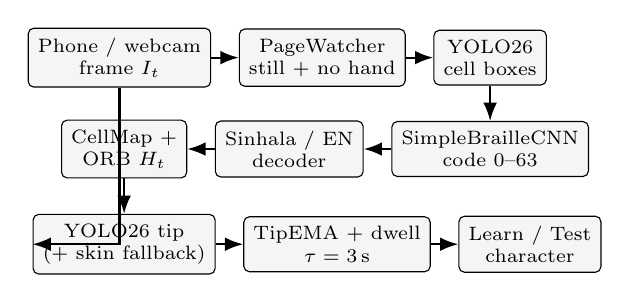
\begin{tikzpicture}[
  font=\scriptsize,
  box/.style={draw, rounded corners=2pt, align=center, inner sep=3.5pt, fill=gray!8},
  arr/.style={-{Latex}, thick}
]
\node[box] (cam) {Phone / webcam\\frame $I_t$};
\node[box, right=0.35cm of cam] (watch) {PageWatcher\\still + no hand};
\node[box, right=0.35cm of watch] (yolo) {YOLO26\\cell boxes};
\node[box, below=0.45cm of yolo] (cnn) {SimpleBrailleCNN\\code $0$--$63$};
\node[box, left=0.35cm of cnn] (dec) {Sinhala / EN\\decoder};
\node[box, left=0.35cm of dec] (map) {CellMap +\\ORB $H_t$};
\node[box, below=0.45cm of map] (tip) {YOLO26 tip\\(+ skin fallback)};
\node[box, right=0.35cm of tip] (dwell) {TipEMA + dwell\\$\tau=3\,\mathrm{s}$};
\node[box, right=0.35cm of dwell] (out) {Learn / Test\\character};
\draw[arr] (cam) -- (watch);
\draw[arr] (watch) -- (yolo);
\draw[arr] (yolo) -- (cnn);
\draw[arr] (cnn) -- (dec);
\draw[arr] (dec) -- (map);
\draw[arr] (cam) |- (tip);
\draw[arr] (map) -- (tip);
\draw[arr] (tip) -- (dwell);
\draw[arr] (dwell) -- (out);
\end{tikzpicture}
\caption{BrailleLens at inference. Cell detection and classification run
once per captured page; fingertip tracking runs every frame. Language
decoding is a lookup, not a second network.}
\label{fig:arch}
\end{figure}

A second, slower path remains as a baseline: classical or YOLO
\textit{dot} centres $\rightarrow$ grid clustering $\rightarrow$ the same
CNN. We use it for ablation and for pages where a cell-detector checkpoint
is missing.

\section{Data Engineering}
\label{sec:data}

\subsection{Sources}
\textbf{DSBI}~\cite{li2018dsbi} contributes 91{,}443 cells on 220 flatbed
pages (114 page groups), all 64 codes present, median box $36\times 58$~px
and median dot pitch 28.9~px. \textbf{Angelina}~\cite{ovodov2021obr}
contributes 66{,}116 cells on 212 handheld photographs, 54 of 64 codes,
median box $22\times 33$~px and pitch 16.5~px. \textbf{Gold} is our own
Sinhala book: 12 physical pages photographed under high and low lighting.
Only the high-quality twin is labelled in LabelMe (dot-number strings such
as \texttt{1345}); boxes transfer to the low-quality twin by ORB+RANSAC.
High/Low twins share a \texttt{page\_group} so they cannot leak across
splits. Pages 1--8 train, 9 and 12 validate, and 10--11 are held out for
test (see each experiment's protocol).

\subsection{Contract, cleaning, and crops}
Every cell becomes one row of \texttt{manifest\_clean.csv}: source, path,
page group, split, box, integer code, and measured pitch. Cleaning
retained all 157{,}559 integrated rows (decorative divider rows are
flagged, not dropped by default). Official DSBI has no validation split
and official Angelina has no test split; for training we therefore
rebalance 70/15/15 \textit{by page group}, yielding 120{,}809 / 21{,}095 /
15{,}655 cells with zero page groups spanning two splits.

Crops are $64\times 64$ uint8 grayscale. Source-specific margins matter:
an Angelina box is $\approx 2\,d_x$ by $3\,d_y$, whereas a DSBI-style
asymmetric crop starves the CNN of $\sim$40\% of the area it was trained
on and can cost tens of accuracy points end-to-end
(Section~\ref{sec:exp-angelina}). Each crop is mean--std normalised with
a standard-deviation floor of 10 so blank cells are not amplified into
false contrast.

\subsection{Class imbalance}
On Angelina the most frequent code holds 9.3\% of cells and the present-class
ratio is $6150\times$; ten codes never appear. DSBI is milder (4.7\%,
$26\times$, all 64 codes). Training therefore uses class weights and an
optional per-class cap.

\subsection{Fingertip images}
Generic pretraining uses TI1K and related tip-box sets~\cite{ti1k}.
Domain adaptation uses 60 LabelMe photographs of a real finger on Sinhala
Braille paper, exported to Ultralytics layout as 48 / 6 / 6
(train / val / test, seed 42). The labelled class is a single
\texttt{fingertip} box on the distal pad---the contact that should hit a
cell---not the knuckle or nail.

\section{Methods}
\label{sec:methods}

\subsection{Cell detection}
\label{sec:cells}
The cell detector is a COCO-pretrained YOLO26 nano~\cite{yolo-ultralytics},
fine-tuned as a single class \texttt{braille\_cell}. Input resolution is
1280~px so a DSBI cell that is $\sim$36~px tall remains $\sim$27~px after
resize (at 640~px it would shrink to $\sim$14~px). \texttt{max\_det}=800
covers the measured maximum of 623 cells/page. Photometric augmentation is
aggressive (HSV, exposure) because the domain gap is mostly lighting;
geometric augmentation is mild (3$^\circ$ rotation, small shear/perspective)
because axis-aligned labels inflate under large rotation. Horizontal and
vertical flips are disabled: on the 12-image Gold set they collapsed
validation mAP$_{50}$ from 0.81 to 0.32---too much variance for that
little data. Mosaic is 0.5; mixup is 0 because blending two dense pages
invents false cells.

Gold-domain fine-tuning adds the low-lighting twins and
shear/perspective, then (optionally) a \textit{spine-boost} second pass:
the detector is re-run on an upscaled strip nearest the book spine, where
cells are uniformly $\sim$6--7\% smaller from page curvature, and boxes
are merged by NMS. Decorative ruler rows are removed after
classification by a code-diversity test (Section~\ref{sec:exp-gold}).

\subsection{Cell classification}
\label{sec:cnn}
SimpleBrailleCNN is a three-block network:
\begin{equation}
\begin{aligned}
&\mathrm{Conv}(1\!\to\!16)\!\to\!\mathrm{BN}\!\to\!\mathrm{ReLU}\!\to\!\mathrm{MaxPool},\\
&\mathrm{Conv}(16\!\to\!32)\!\to\!\mathrm{BN}\!\to\!\mathrm{ReLU}\!\to\!\mathrm{MaxPool},\\
&\mathrm{Conv}(32\!\to\!64)\!\to\!\mathrm{BN}\!\to\!\mathrm{ReLU}\!\to\!\mathrm{MaxPool},\\
&\mathrm{AdaAvgPool}(4)\!\to\!\mathrm{FC}(1024,128)\!\to\!\mathrm{Dropout}(0.3)\\
&\qquad\!\to\!\mathrm{FC}(128,64).
\end{aligned}
\end{equation}
Input is $(B,1,64,64)$ in $[0,1]$ after per-crop normalisation. The
model has on the order of $1.6\times 10^5$ parameters---small enough for
CPU live use and for mixed-domain fine-tuning without catastrophic
overfitting of a huge backbone.

Training schedule used in this work:
\begin{itemize}
\item synthetic renderer (Gaussian-bump dots, rotation, optional
perspective warp) $\rightarrow$ \texttt{braille\_cnn\_best.pt};
\item DSBI fine-tune, Adam $10^{-4}$, 10 epochs $\rightarrow$
\texttt{braille\_cnn\_dbsi\_finetuned.pt};
\item mixed synthetic+DSBI+Angelina batches $\rightarrow$
\texttt{braille\_cnn\_angelina\_finetuned.pt} /
\texttt{braille\_cnn\_mixed.pt}, which avoids the catastrophic
forgetting observed when DSBI-only fine-tuning is evaluated back on
synthetic cells (14\%);
\item Gold fine-tune mixed with live DSBI crops $\rightarrow$
\texttt{braille\_cnn\_gold\_finetuned.pt}.
\end{itemize}

A separate DotPatchCNN ($32\times 32$ binary verifier) is trained on
detector-anchored positives and hard negatives (including verso
bleed-through) to raise classical-dot precision from $\sim$50\% to
$\sim$99\% on scanner pages. It is a baseline component, not the live
default.

\subsection{Language decoding}
\label{sec:decode}
Given a sequence of codes, \texttt{decode\_sequence} runs two passes.
Pass 1 consumes indicator 60 (short-vowel) or 61 (long-vowel) plus the
next modifier and emits a combining sign or independent long vowel.
Pass 2 maps remaining codes through \texttt{CODE\_TO\_SINHALA} (63 unique
non-zero glyphs: independent vowels, five vargas, semivowels, sibilants,
and diacritics). Combining marks in U+0DCA--U+0DDF append to the previous
consonant so a Unicode renderer composes, e.g., \textit{ka}+\textit{aa}
$\rightarrow$ \textit{kaa}. English is the same visual codes with a
different lookup table. Low-confidence cells may be emitted as a
placeholder rather than a guess.

Word spaces are not detected as boxes---an all-blank cell has no raised
dots. We insert synthetic space tokens where the within-line $x$-gap
exceeds $\approx 1.6\times$ the median cell pitch. Attempting to
\textit{classify} those implied slots made page accuracy worse
(softmax overconfidence on empty crops) and was rejected.

\subsection{Fingertip tracking}
\label{sec:tip}
Three detectors share one factory.

\paragraph{YOLO26n (default).}
\texttt{TipYOLO} runs a single-class YOLO26 nano on the live frame and
returns the highest-confidence box centre. Weights resolve in order:
the Braille-domain checkpoint
\texttt{yolo26n\_fingertip\_braille\_best.pt} (fine-tuned from a generic
fingertip YOLO26n on the 60-image set), then the generic
\texttt{yolo26n\_fingertip\_best.pt}. This is the live default because
it is trained to fire on a distal pad over Braille texture, does not
need a visible palm, and produces a box the HUD can draw.

\paragraph{SkinContourTip (fallback).}
If YOLO returns no box, a classical pipeline runs the same frame: YCrCb
in-range mask with a brightness cap so cream paper is not called skin;
morphological open/close; contour filter (area, solidity, thickness,
border entry, corner ghosts, reach into the page); contact point on the
distal 20\% of the contour, pulled slightly toward the wrist so the pad
rather than the nail hits the cell. This path has no neural net, is
robust when the palm is cropped, and fails independently of YOLO (e.g.\
motion blur that empties the detector can still leave a blob).

\paragraph{MediaPipe Hands (optional).}
Landmark 8, pulled back toward MCP 5, remains available as
\texttt{--tip-backend mediapipe}. It is not the default: over-page
Braille footage routinely hides the palm.

\paragraph{Temporal association.}
TipEMA applies an exponential moving average
$p \leftarrow \alpha p_{\mathrm{raw}} + (1-\alpha)p$ with $\alpha=0.35$,
rejects jumps beyond 180~px until the previous track has been lost for
eight frames, and coasts up to five frames on a miss. A dwell filter
then requires the same CellMap id for $\tau=3000$~ms before a character
is printed, which is essential for a learning app (a sliding finger
would otherwise chatter).

\subsection{Page capture and registration}
\label{sec:reg}
PageWatcher is a four-state machine (SEARCHING $\rightarrow$ CAPTURING
$\rightarrow$ TRACKING $\rightarrow$ SEARCHING). Capture fires when
motion (mean absolute grey difference) stays below a threshold for a
streak of frames, the tip backend reports no hand, a cooldown has
elapsed, and the scan yields enough cells at sufficient confidence.
Manual \texttt{R} remains an override.

Cell boxes live in the scan's reference frame. Live frames drift, so
\texttt{FrameRegistration} estimates a homography from ORB features
(2000 keypoints, Hamming BFMatcher, Lowe ratio 0.75, RANSAC 5~px).
Whole-page matching is used on purpose: the fingertip occludes local
texture exactly where a patch tracker would look. A single failed frame
does not drop the map; consecutive failures mark registration LOST and
return the watcher to SEARCHING. Display boxes are the axis-aligned
hull of the four corners mapped by $H^{-1}$.

\subsection{Interaction modes}
Learning mode announces a cell the first time it is dwelt, keyed by
session memory so a fidget does not repeat. Testing mode prompts for a
typed character and scores it. Sinhala is the default language of the
live app.

\begin{algorithm}[t]
\caption{Per-frame live loop (simplified)}
\label{alg:live}
\begin{algorithmic}[1]
\State $p,\,b,\,s \gets \mathrm{YOLO26\_tip}(I_t)$
\If{$p=\emptyset$}
  \State $p,\,b,\,s \gets \mathrm{SkinContour}(I_t)$ \Comment{fallback}
\EndIf
\State $p \gets \mathrm{TipEMA}(p)$
\If{page not captured \textbf{and} still \textbf{and} no hand}
  \State $\mathrm{CellMap} \gets \mathrm{recognize\_page}(I_t)$
  \State $\mathrm{ORB.reset}(I_t)$
\EndIf
\State $H_t \gets \mathrm{ORB.homography\_or\_last}(I_t)$
\State $\tilde{p} \gets H_t p$ \Comment{into scan frame}
\State $\mathrm{cell} \gets \mathrm{hit\_test}(\tilde{p},\mathrm{CellMap})$
\If{$\mathrm{dwell}(\mathrm{cell},\tau)$}
  \State announce or quiz $\mathrm{cell}.\mathrm{char}$
\EndIf
\end{algorithmic}
\end{algorithm}

\section{Experiments}
\label{sec:exp}

Unless noted, classifier metrics are top-1 accuracy on ground-truth
crops (isolating recognition from detection). Detector metrics are
precision, recall, and mAP$_{50}$ at IoU 0.5. End-to-end page metrics
compare decoded letters against transcribed Gold text after filtering
to a--z and space.

\subsection{Synthetic-to-scanner domain gap}
\label{sec:exp-dbsi}
Table~\ref{tab:cnn} records the central classification result. A
synthetic-only CNN is perfect on its own test distribution and only
51.2\% on 71{,}250 DSBI test cells (chance $\approx$1.6\%), with errors
concentrated on 4+ dot patterns. Fine-tuning on 20{,}193 DSBI train
cells for 10 epochs reaches 98.44\%. Per-crop normalisation then
improves DSBI to 99.24\% at a small synthetic cost (100\% $\rightarrow$
98.85\%): the network can no longer shortcut on absolute brightness.
Recto (98.24--99.33\%) and verso (98.65--99.16\%) are statistically
similar; the folklore that verso is ``harder'' does not hold on this
scanner set. Residual errors on code 18 (dots 2,5) trace to faint
physical marks that annotators treated as absent---a label-noise floor,
not a cropping bug (the mark survives a tighter margin).

\begin{table}[t]
\caption{SimpleBrailleCNN cell accuracy (ground-truth crops).}
\label{tab:cnn}
\centering
\begin{tabular}{lcc}
\toprule
Checkpoint / protocol & Domain & Acc. (\%) \\
\midrule
Synthetic only, synthetic test & synth & 100 \\
Synthetic only, DSBI test (zero-shot) & scan & 51.2 \\
DSBI fine-tuned, DSBI test & scan & 98.44 \\
+ per-crop normalisation, DSBI test & scan & \textbf{99.24} \\
\quad recto / verso & scan & 99.33 / 99.16 \\
Mixed (synth+DSBI+Angelina), DSBI & scan & 98.88 \\
Mixed, Angelina GT boxes & phone & 99.8--100 \\
Mixed, synthetic test & synth & 93.18 \\
Gold baseline (\texttt{mixed.pt}), Gold test & Sinhala & 67.74 \\
Gold fine-tuned, Gold test pages 10--11 & Sinhala & \textbf{95.93} \\
\bottomrule
\end{tabular}
\end{table}

Perspective warp of synthetic cells drops the synthetic-only checkpoint
from 99.97\% to 87.47\%. The DSBI-only fine-tune scores $\sim$14\% on
synthetic images \textit{with or without} warp: it has forgotten the
source domain. Mixed-domain batches are the remedy we adopt for later
checkpoints.

\subsection{Why cell YOLO, not dots}
\label{sec:exp-angelina}
On held-out DSBI pages, local $z$-score peaks, DotPatchCNN verification,
a calibrated peak-$y$ offset, and grid assignment raise end-to-end cell
accuracy from $\sim$25\% to 73.9--97.4\%, with a column-phase ambiguity
fix recovering $\sim$67 points on one page (30.1\% $\rightarrow$ 97.4\%).
Those calibrations are scanner-specific.

On a held-out Angelina photograph the same chain started at $\sim$0--10\%.
Scale-adaptive pitch search and a tight $d_x\!\approx\!d_y$ window (to
avoid locking onto the inter-cell gap $P_x-d_x$ or its $2\times$
harmonic) plus an Angelina-shaped crop box raised end-to-end accuracy to
43.2\% (127/169 cells matched, 73 correct). About 25\% of true cells
still received no cluster, and matched-but-wrong cells had 9.3~px mean
centring error versus 3.6~px for correct ones. Classification of
ground-truth Angelina boxes is essentially solved (Table~\ref{tab:cnn});
the remaining error is localisation. Whole-cell YOLO is therefore the
deployment detector: it predicts the box the CNN and the fingertip
hit-test both need, without a page-global lattice.

\subsection{Sinhala Gold pages}
\label{sec:exp-gold}
\paragraph{Classifier.}
On held-out Gold test pages (ground-truth crops, never used for
checkpoint selection), mixed-domain weights score 67.74\%. Fine-tuning
on pages 1--8 mixed with DSBI crops, selecting on pages 9 and 12, reaches
95.93\% on pages 10--11 (Table~\ref{tab:cnn}). DSBI subset accuracy stays
at 99.4\%---no regression.

\paragraph{Detector.}
Table~\ref{tab:det} shows cell-detector mAP on the same held-out pages.
The public-domain cell checkpoint is a weak prior for our book (mAP$_{50}$
0.41). Gold fine-tuning without shear/perspective reaches 0.65; adding
those augmentations on a GPU with low-light twins reaches \textbf{0.80}
(precision 0.75, recall 0.76). A CPU-only attempt without mosaic stalled
at mAP$_{50}$ 0.38, confirming that this detector needs both in-domain
photos and adequate augmentation.

\begin{table}[t]
\caption{Cell detector on held-out Gold pages 10--11 (max\_det=800).}
\label{tab:det}
\centering
\begin{tabular}{lccc}
\toprule
Model & mAP$_{50}$ & P & R \\
\midrule
\texttt{braille\_cell\_best.pt} & 0.409 & 0.558 & 0.481 \\
Gold FT, no shear/perspective & 0.653 & 0.730 & 0.744 \\
Gold FT + shear/perspective & \textbf{0.795} & \textbf{0.746} & \textbf{0.757} \\
\bottomrule
\end{tabular}
\end{table}

\paragraph{Spine foreshortening.}
Misses are not random and are not a brightness problem (missed cells are
slightly \textit{brighter}). They cluster at line starts nearest the
spine and are 6--7\% smaller at unchanged aspect ratio---page curl, not
shadow. At confidence 0.02, 94--97\% of ``misses'' have a matching raw
box: the signal exists but scores below the 0.30 operating point. A
global size-adaptive threshold and CLAHE both hurt F1. A
\textit{targeted} second pass on the spine strip
(\texttt{spine\_strip\_frac}=0.45, $2\times$ upscale) raises F1 from
0.742 to 0.761; upscaling the \textit{whole} page only reaches 0.747.
The gain is regional, not a resolution trick.

\paragraph{Ruler rows.}
Decorative divider lines are unlabelled by design and look like a row of
cells. Confidence cannot separate them from sparse true lines. After
CNN codes are assigned, a line of $\ge$15 cells whose top-two codes
cover $\ge$55\% of the line is dropped. On all 12 Gold pages this never
removes a matched true cell; it fires on two pages and is pure precision
gain (e.g.\ page 11 F1 0.748 $\rightarrow$ 0.779).

\paragraph{End-to-end text.}
Table~\ref{tab:e2e} reports letters-only accuracy against human
transcriptions of six Gold pages (capital/number/punctuation ids
skipped as unverified). With cell confidence 0.30, spine-boost, and
ruler drop: overall \textbf{79.3\%} letters-only and 61.6\% with spaces.
Space accuracy is structurally lower because YOLO does not propose empty
word-gap boxes; geometric gap insertion recovers some but not all.

\begin{table}[t]
\caption{End-to-end Gold page accuracy (\texttt{recognize\_page}, cells
backend, English letter filter).}
\label{tab:e2e}
\centering
\begin{tabular}{lcccc}
\toprule
Page & Cells & GT chars & Acc.\ (spaces) & Acc.\ (letters) \\
\midrule
pg-1 & 348 & 290 & 0.603 & 0.764 \\
pg-2 & 296 & 238 & 0.660 & 0.863 \\
pg-3 & 329 & 276 & 0.627 & 0.805 \\
pg-4 & 391 & 290 & 0.569 & 0.797 \\
pg-5 & 314 & 264 & 0.576 & 0.727 \\
pg-6 & 332 & 287 & 0.669 & 0.807 \\
\midrule
Overall & --- & --- & 0.616 & \textbf{0.793} \\
\bottomrule
\end{tabular}
\end{table}

Ideas we tried and rejected, with the same split: lower NMS IoU (Ovodov's
0.02), which does nothing on this anchor-free head; \texttt{fliplr}/
\texttt{flipud}; classify-based grid-gap recovery; global small-box
thresholds; CLAHE.

\subsection{Fingertip YOLO26}
\label{sec:exp-tip}
The Braille-domain fine-tune starts from
\texttt{yolo26n\_fingertip\_best.pt}, 80 epochs, mosaic 0.5, mixup 0.05,
\texttt{fliplr} 0.5 (safe here: a mirrored fingertip is still a
fingertip). Table~\ref{tab:tip} reports the exported metrics. Precision,
recall, and mAP$_{50}$ saturate on both the 6-image val and 6-image test
splits; mAP$_{50:95}$ (0.65 val / 0.70 test) is the more honest
localisation score. We treat mAP$_{50}=0.995$ as an \textit{upper bound}
on a tiny in-domain set, not as a claim of perfect video tracking, and
we therefore keep SkinContourTip as a per-frame fallback in the live
app rather than shipping YOLO alone.

MediaPipe Hands is retained as an ablation backend. On top-down
over-page recordings it is expected to fail whenever the palm is out of
frame---the operating regime of a learner touching a book---which is why
it is not the default cascade.

\begin{table}[t]
\caption{YOLO26n fingertip fine-tune on 60 Braille photographs
(48/6/6). Metrics from the training export.}
\label{tab:tip}
\centering
\begin{tabular}{lcccc}
\toprule
Split & P & R & mAP$_{50}$ & mAP$_{50:95}$ \\
\midrule
Val (6 images) & 1.00 & 1.00 & 0.995 & 0.647 \\
Test (6 images) & 1.00 & 1.00 & 0.995 & 0.700 \\
\bottomrule
\end{tabular}
\end{table}

\subsection{Live system}
The live loop (Algorithm~\ref{alg:live}) is CPU-runnable in the Stage~5
venv (PyTorch + Ultralytics + OpenCV). Auto-scan is on by default.
Registration was validated under synthetic rotation, translation, scale,
and $\sim$25\% occlusion with sub-pixel mapping error. A Flutter ONNX
path exists as a prototype (quantised YOLO26n fingertip export); the
evaluated research system is the Python pipeline.

\section{Discussion}
\label{sec:discuss}

\paragraph{Decouple vision from language.}
A 64-way visual code plus a lookup table let us correct Sinhala labels
without a retrain and run English evaluation on Sinhala photographs
(Table~\ref{tab:e2e}). Two-cell vowel signs never enter the CNN.

\paragraph{Detect the object you will hit-test.}
Dot clustering can be made to work on scans; it is the wrong abstraction
for a fingertip app. Cell boxes are both the CNN crop and the dwell
target.

\paragraph{Domain gaps compound.}
Synthetic $\rightarrow$ scanner (51\% $\rightarrow$ 99\%), scanner
$\rightarrow$ handheld grid (97\% $\rightarrow$ 43\% e2e), mixed CNN
$\rightarrow$ Sinhala Gold crops (68\% $\rightarrow$ 96\%), public cell
YOLO $\rightarrow$ Gold pages (mAP 0.41 $\rightarrow$ 0.80). Each gap
needed its own data, not a bigger backbone. Catastrophic forgetting
appeared the moment we fine-tuned on one domain only.

\paragraph{Small in-domain sets still move the needle---with caveats.}
Twelve Gold pages and 60 fingertip photos are enough to change the
operating point of a pretrained detector, but they are not enough for
flip augmentation (Gold cells) and not enough to trust saturated
mAP$_{50}$ (fingertips). The cascade YOLO $\rightarrow$ skin is the
engineering response to that uncertainty: the network is the default
because it is in-domain; the contour tracker covers misses without a
second GPU model.

\paragraph{Open books are not flat scans.}
Spine curl suppresses confidence, not contrast. Divider rows fool box
geometry. Both were diagnosed with overlays and fixed with
\textit{targeted} rules rather than a lower global threshold.

\paragraph{Limitations.}
(1)~End-to-end Gold letters-only accuracy is 79\%, not classroom-ready
for unsupervised transcription; the interactive dwell task is more
forgiving because the learner chooses one cell. (2)~The fingertip test
split is six images; a labelled video benchmark is future work.
(3)~Sinhala vowel-indicator decoding is implemented and table-checked
but the published Gold text metric uses an English letter filter.
(4)~The Flutter on-device stack is not the evaluated system.
(5)~Native-speaker review of \texttt{CODE\_TO\_SINHALA} is still required
before any TTS deployment.

\section{Conclusion}
\label{sec:conc}

BrailleLens is a complete OBR-plus-learning stack for Sinhala Braille
photographed by a handheld camera. A YOLO26 cell detector and a compact
64-class CNN, trained through a leakage-safe multi-source pipeline and
fine-tuned on a small Gold set, support a live reader whose default
fingertip model is a Braille-domain YOLO26n detector with a classical
skin-contour fallback. The main scientific lessons are practical:
keep language out of the visual softmax; detect cells rather than
reconstructing them from dots when the user will point at a box; treat
each capture domain as a separate adaptation problem; and pair a small
in-domain network with a cheap, independent fallback instead of
pretending a six-image test set is a solved tracker.

Future work is a larger fingertip video benchmark, gold-text evaluation
in Sinhala (including two-cell vowels), tighter spine-aware training,
and a single on-device runtime that fuses the ONNX cell, CNN, and
fingertip models already exported from this codebase.

\section*{Acknowledgment}
This work was carried out as the CS3501 Data Science and Engineering
Project (Group 15). We thank the authors of DSBI~\cite{li2018dsbi} and
the Angelina / OBR-CNN work~\cite{ovodov2021obr} for the public corpora
that make the transfer-learning path possible, and Ultralytics for the
YOLO26 training stack~\cite{yolo-ultralytics}.

\begin{thebibliography}{00}

\bibitem{li2018dsbi}
R.~Li, H.~Liu, X.~Wan, and Y.~Qian, ``DSBI: Double-sided Braille image
dataset and algorithm evaluation for Braille dots detection,''
\textit{arXiv:1811.10804}, 2018.

\bibitem{ovodov2021obr}
I.~G.~Ovodov, ``Optical Braille recognition using object detection CNN,''
in \textit{Proc.\ IEEE/CVF Int.\ Conf.\ Computer Vision Workshops
(ICCVW)}, 2021, pp.~1741--1748.

\bibitem{lu2022anchor}
L.~Lu, D.~Wu, J.~Xiong, Z.~Liang, and F.~Huang, ``Anchor-free Braille
character detection based on edge feature in natural scene images,''
\textit{Computational Intelligence and Neuroscience}, vol.~2022,
Art.~7201775.

\bibitem{ahn-dotneuralnet}
Y.~J.~Ahn \textit{et al.}, ``Connect the dots / DotNeuralNet: YOLO models
for Braille symbol detection,'' open-source implementation, used as a
baseline cell detector in this work.

\bibitem{yolo-ultralytics}
G.~Jocher, J.~Qiu, and A.~Chaurasia, ``Ultralytics YOLO,'' 2023--2026.
[Online]. Available: \url{https://github.com/ultralytics/ultralytics}

\bibitem{mediapipe-hands}
F.~Zhang \textit{et al.}, ``MediaPipe Hands: On-device real-time hand
tracking,'' \textit{arXiv:2006.10214}, 2020.

\bibitem{ti1k}
M.~Alam \textit{et al.}, ``TI1K: A dataset for fingertip detection,''
GitHub repository.
[Online]. Available: \url{https://github.com/MahmudulAlam/TI1K-Dataset}

\bibitem{unicode-sinhala}
Unicode Consortium, ``Sinhala,'' in \textit{The Unicode Standard},
and Sri Lanka Braille usage notes for Grade-1 cells and combining
vowel indicators.

\bibitem{redmon2016yolo}
J.~Redmon, S.~Divvala, R.~Girshick, and A.~Farhadi, ``You only look
once: Unified, real-time object detection,'' in \textit{Proc.\ IEEE
Conf.\ Computer Vision and Pattern Recognition (CVPR)}, 2016.

\bibitem{he2016resnet}
K.~He, X.~Zhang, S.~Ren, and J.~Sun, ``Deep residual learning for image
recognition,'' in \textit{Proc.\ IEEE Conf.\ Computer Vision and Pattern
Recognition (CVPR)}, 2016.

\bibitem{ioffe2015bn}
S.~Ioffe and C.~Szegedy, ``Batch normalization: Accelerating deep
network training by reducing internal covariate shift,'' in
\textit{Proc.\ Int.\ Conf.\ Machine Learning (ICML)}, 2015.

\bibitem{lowe2004sift}
D.~G.~Lowe, ``Distinctive image features from scale-invariant
keypoints,'' \textit{Int.\ J.\ Computer Vision}, vol.~60, no.~2,
pp.~91--110, 2004.

\bibitem{rublee2011orb}
E.~Rublee, V.~Rabaud, K.~Konolige, and G.~Bradski, ``ORB: An efficient
alternative to SIFT or SURF,'' in \textit{Proc.\ IEEE Int.\ Conf.\
Computer Vision (ICCV)}, 2011.

\bibitem{fischler1981ransac}
M.~A.~Fischler and R.~C.~Bolles, ``Random sample consensus: A paradigm
for model fitting with applications to image analysis and automated
cartography,'' \textit{Commun.\ ACM}, vol.~24, no.~6, pp.~381--395, 1981.

\bibitem{szegedy2015inception}
C.~Szegedy, W.~Liu, Y.~Jia \textit{et al.}, ``Going deeper with
convolutions,'' in \textit{Proc.\ IEEE Conf.\ Computer Vision and
Pattern Recognition (CVPR)}, 2015.

\bibitem{lin2017focal}
T.-Y.~Lin, P.~Goyal, R.~Girshick, K.~He, and P.~Doll\'{a}r, ``Focal
loss for dense object detection,'' in \textit{Proc.\ IEEE Int.\ Conf.\
Computer Vision (ICCV)}, 2017.

\bibitem{bochkovskiy2020yolov4}
A.~Bochkovskiy, C.-Y.~Wang, and H.-Y.~M.~Liao, ``YOLOv4: Optimal speed
and accuracy of object detection,'' \textit{arXiv:2004.10934}, 2020.

\end{thebibliography}

\end{document}
